\documentclass[psamsfonts,onesided,10pt]{amsart}
\usepackage{goodstyle}


%opening
\title{HW 2 - Write Up}
\author{Robin Belton, Daniel Laden, Jiahui Ma,  Badr Zerktouni}

\begin{document}

\maketitle

\section{System Usage}
\subsection{System Setup}
This system was written with Python version 3.7. The system depends on the following python packages.

\begin{itemize}
    \item pandas
    \item numpy
    \item itertools 
    \item random
\end{itemize}

\subsection{Running the System}
This system uses Iris Data csv located at \path{https://github.com/jiahuiblair/CSCI-550-HW2/iris.csv} 
to test clustering and assessment algorithms. All python functions are included in the \path{main.py} file \todo{create this}

All functions can be run in the command line as follows:

\begin{description}
\item[Synthetic Data] To generate synthetic data where $(x,y)$ points are sampled from 
non-overlapping rectangular regions, run \textsc{SyntheticRectData}$(k,n,r)$ where $k$ is the 
number of points to sample from $n$ non-overlapping rectangular regions in $\mathbb{R}^2$. 
The noise parameter, $r$  is the number of noise points to add to the data that is not in the interior 
of any rectangular region. The output will be a data frame with attributes, `X', `Y', and `Label'. 
`X' and `Y' denote the $x-,y-$coordinates of the data point and the label denotes which rectangle 
the point was sampled from. A label of zero means the point is added noise.
\item[$k$-means] \todo{}
\item[DBSCAN] \todo{}
\item[Purity]  To compute the purity of a clustered data set, $C$, to a given partition, $D$ run 
\textsc{Purity}$(D, C, n)$. $C$ and $D$ need to be data frames with 
attributes `X',  `Y', and `Label'. Additionally, this function is written for data that has been 
classified in three clusters where the labels of the clusters are either 1, 2, or 3. 
\item[Silhouette] \todo{}
\end{description}
 
\section{Example of Input/Output}
\begin{description}
\item[Synthetic Data] Below we run the SyntheticRectData for sampling 30 points from 3 
rectangular regions with 10 noise points. We also plot the results.
\begin{verbatim}
synth = SyntheticRectData(30,3,10)
plt.plot(synth['X'][0:29], synth['Y'][0:29], 'ro', #plot results
         synth['X'][30:59], synth['Y'][30:59], 'bo', 
         synth['X'][60:89], synth['Y'][60:89], 'go',
         synth['X'][90:99], synth['Y'][90:99], 'yo')
plt.show()   
\end{verbatim}
\begin{figure}[H]
    \centering
    {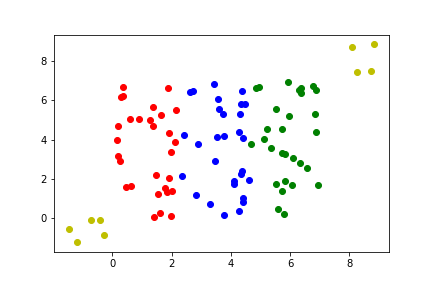
\includegraphics[width=.4\textwidth]{images/synth.png}} \\
    \caption{Plotting output of synth. Red, blue, and green represent the three rectangular regions. 
Yellow points are the added noise.}
\end{figure}
\item[$k$-means] \todo{}
\item[DBSCAN] \todo{}
\item[Purity] Below we first produce the ground truth data for the Iris data set using Sepal Length 
and Sepal Width as the X and Y attributes. We then apply purity to the $k$-means output when $e=0.05$. 
\begin{verbatim}
D = iris[['Sepal Length', 'Sepal Width', 'Species']]
ground_truth = np.zeros((len(D.iloc[:,0]),3))
ground_truth[:,0] = D.iloc[:,0]
ground_truth[:,1] = D.iloc[:,1]
for i in range(len(D.iloc[:,0])):
    if D.iloc[i,2]=='Iris-setosa':
        ground_truth[i,2] = 1
    elif D.iloc[i,2]=='Iris-versicolor':
        ground_truth[i,2] = 2
    else:
        ground_truth[i,2] = 3
groundtruth = pd.DataFrame({'X':ground_truth[:,0], 'Y':ground_truth[:,1], 
                 'Label':ground_truth[:,2]})       
# Compute purity with Kmeans output, km (need to run k-means clustering function to get km)
Purity(groundtruth, km, 150)
# output = 0.66
\end{verbatim}
\item[Silhouette] \todo{}
\end{description}

\section{Exploring Datasets}
In this section we describe our findings from Part 4. \todo{}

\end{document}
